\chapter{Ознакомительная}
\textbf{Цель:} Запустить плату, подключиться к ней через консоль и по сетевому интерфейсу, работа с кнопкой и светодиодами через sysfs.

\vspace{5mm}
\textbf{Описание:} работа с ОС Linux на целевой платформе мало чем отличается от работы с данной ОС на обычном компьютере. Среди особенностей можно выделить наличие меньшего набора инструментов, и рабочих программ, что делается для экономии свободного места, и ускорения загрузки ОС. Так же может отсутствовать привычный рабочий стол, а вся работа сводиться к взаимодействию через рабочий терминал, она же консоль. Для подключения к консоли можно воспользоваться интерфейсом UART (он же COM порт, или последовательный порт), или при помощи сетевого соединения (ssh или реже telnet). 

При этом нужно понимать, что возможность работы через консоль настраивается, и не всегда может быть доступна по-умолчанию (обычно возможность сетевого подключения отключают, для повышения безопасности). 


\section{Запуск и подключение к устройству}

\subsection{}Запустите виртуальную машину. Логин и пароль для входа: student / usrstudent.

\subsection{}Подключите по USB плату к ПК. Проверьте, и при необходимости подключите USB устройство FTDI RBM\_C1K5500VK018 к виртуальной машине (меню Device→USB).

\subsection{}Откройте программу gtkterm, и подключитесь к порту /dev/ttyUSB1

\subsection{}Если в окне терминала нет текста, нажмите клавишу Enter на клавиатуре. Вы должны увидеть следующий вывод:
\begin{center}
	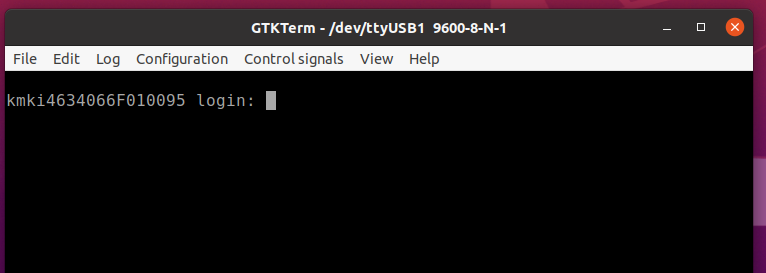
\includegraphics[width=\textwidth]{pic_08}
\end{center}
Вы подключились к консоли устройства. Введите логин root и пароль root.

\section{Подключение по сетевому интерфейсу}

Рассмотрим какие шаги необходимо выполнить, для того, что бы можно было организовать сетевое подключение к плате, для получение доступа к консоли, и файловой системе через SSH соединение. Так же настройки, которые будут выполнены в данном разделе помогут в дальнейшем копировать файлы на плату через команду scp.

\subsection{}Проверьте текущие настройки интерфейса eth0 выполнив команду: 
\begin{lstlisting}[style=bash]
$ ip addr show dev eth0 
\end{lstlisting}
Вы должны увидеть, что выдаче появилась строчка: 
\begin{lstlisting}[style=stdout]
	...
inet 192.168.100.200/24 scope global eth0 
	...
\end{lstlisting}
Если inet адрес отличается, то удалите текущий адрес (вместо <inet\_val> впишите адрес, который отобразился у вас)
\begin{lstlisting}[style=bash]
$ ip addr del <inet_val> dev eth0
\end{lstlisting}
затем установите новый адрес командой 
\begin{lstlisting}[style=bash]
$ ip addr add 192.168.100.200/24 dev eth0
\end{lstlisting} 
Для активации изменения необходимо переподключиться, для чего выполните следующие команды
\begin{lstlisting}[style=bash]
$ ip link set eth0 down
$ ip link set eth0 up
\end{lstlisting} 

\subsection{}Проверьте, что на плате запущен SSH сервер. Проверить открытые порты устройства, выполнив команду: 

\begin{lstlisting}[style=bash]
$ netstat -tulpn | grep LISTEN
\end{lstlisting} 
\begin{center}
	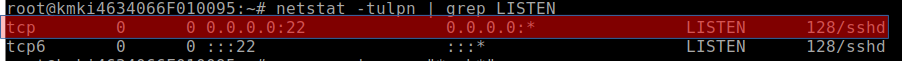
\includegraphics[width=\textwidth]{pic_09}
\end{center}
Если вы не увидели, вывода, как на картинках выше, то выполните команду: 
\begin{lstlisting}[style=bash]
$ systemctl start sshd 
\end{lstlisting}
и проверьте снова. 

\subsection{}\label{lab2:ref1}Заходить через сеть в пользователя root не безопасно, поэтому создадим пользователя для дальнейшей работы, для этого введите следующие команды (пароль для пользователя netuser - usrnetuser):
\begin{lstlisting}[style=bash]
$ useradd -s /bin/bash -m netuser
$ passwd netuser
\end{lstlisting}

Первая команда для создания нового пользователя netuser с созданием домашнего каталога (/home/netuser) и также назначаем для него использовать интерпретатора bash. 

\subsection{}Подключите сетевой шнур к рабочему ПК и плате

\subsection{}Откройте на виртуальной машине консоль, нажав на клавиатуре комбинацию клавиш Ctrl + Alt + T. 

\subsection{}\label{lab2:ref2}В открывшемся окне терминала введите команду: 
\begin{lstlisting}[style=bash]
# ssh netuser@192.168.100.200
\end{lstlisting}

\subsection{}Вам предложат ввести пароль пользователя, вводим тот, что установили в пункте \ref{lab2:ref1} и получаем доступ к терминалу платы.

Если вместо ввода пароля, Вы увидете надпись похожую на:
\begin{lstlisting}[style=stdout]
The authenticity of host '192.168.100.200 (192.168.100.200)' can't be established.
ECDSA key fingerprint is SHA256:+OSEJhr2dIiTvlWZxq5fZ0UFdYYY+egbTgabe6F7zZE.
Are you sure you want to continue connecting (yes/no/[fingerprint])?
\end{lstlisting}
Введите yes и нажмите Enter, и Вам предложат ввести пароль.
\\\\
Если же получите вывод как на картинке ниже
\begin{center}
	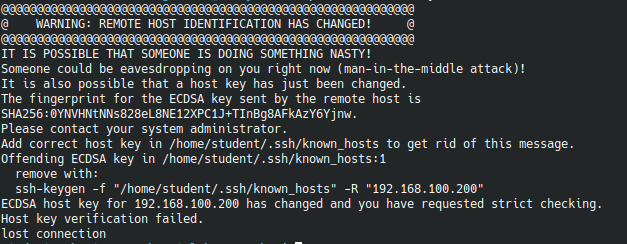
\includegraphics[width=\textwidth]{pic_10}
\end{center}
Выполните команду 
\begin{lstlisting}[style=bash]
$ ssh-keygen -f "/home/student/.ssh/known_hosts" -R "192.168.100.200"
\end{lstlisting}

и вернитесь к пункту \ref{lab2:ref2}

\subsection{}Завершите сеанс, введя команду exit 

\section{Аппаратный Hello world }

В этой части Вы будете управлять выводами микроконтроллера, для переключения светодиодов и считывания состояния кнопки, при помощи виртуальной файловой системы sysfs.

Для работы с периферией в ОС Linux помимо прочего есть две виртуальные файловые системы: procfs (точка входа /proc) и sysfs (точка входа /sys).  

Sysfs экспортирует в пространство пользователя информацию ядра Linux о присутствующих в системе устройствах и драйверах, что позволяет не только считывать значение (например с датчиков температуры), но и менять поведение, если это было заложено разработчиками.

За формирование наполнения виртуальных файловых систем отвечает модуль ядра, который выполняет роль драйвера, если речь идёт про взаимодействие с периферийным модулями (подробно будет рассмотрен в следующих лабораторных работах).

\subsection{}Перейдите в каталог /sys/class/gpio:
\begin{lstlisting}[style=bash]
$ cd /sys/class/gpio
\end{lstlisting}

\subsection{}Выведите список фалов и каталогов в текущей директории: 
\begin{lstlisting}[style=bash]
$ ls -l
\end{lstlisting}
\begin{center}
	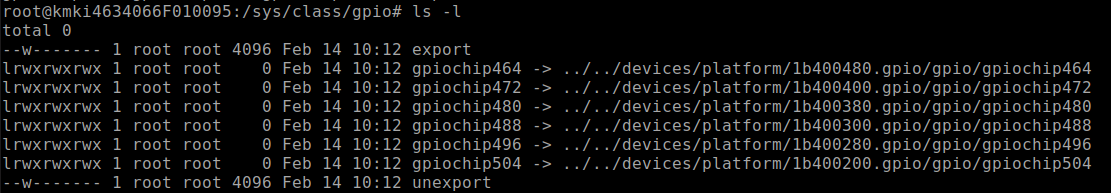
\includegraphics[width=\textwidth]{pic_11}
\end{center}

Разберём то, что Вы видите. Первый и последний файлы используются для того, что бы подключать драйвер для управления отдельным выводом в файловую систему sysfs или отключать. 

Далее идёт серия символьных ссылок на каталоги, каждый из которых описывает один банк сигналов ввода-вывода общего назначения (GPIO). Тут нужно отметить, что в рабочем чипе присутствует 6 банков (A, B, C, D, E и F), по 8 выводов в каждом, по этой причине мы видим 6 каталогов.  

Обратите внимание на имена каталогов, внутри platform. Первая часть имени является базовым адресом периферийного модуля, отвечающего за управление банком выводов. Первому банку выводов A соответствует адрес 0x1B400200, остальные по возрастанию. 

\subsection{}У выводов общего назначения в рамках ядра Linux нумерация сквозная. Таким образом, можно определить, что вывод подключённый к кнопке SW2 находиться под номерам 486.  Выполним следующую команду:
\begin{lstlisting}[style=bash]
$ echo 486 > export
\end{lstlisting}

\subsection{}Выполните эту же команду для экспорта выводов пары выводов банка F (504 и 505) 

\subsection{}После каждой команды будет создан каталог ./gpioXXX где вместо XXX будет номер вывода. Если зайти в любой из этих каталогов, то можно увидеть там одинаковый набор файлов, но нас интересуют следующие: 
\begin{itemize}
\item direction — задаёт направление вывода (in вывод настроен как вход, out — как выход)
\item value — если вывод настроен как вход, то читая этот файл можем узнать уровень логического сигнала на выводе. Если настроен на выход, то запись в этот файл 0 или 1 будет устанавливать соответствующий уровень выходного сигнала.
\end{itemize}

\subsection{}Так как два вывода банка F управляют светодиодами, изменим значение в файле direction  для них на out
\begin{lstlisting}[style=bash]
$ echo out > gpio504/direction
$ echo out > gpio505/direction
\end{lstlisting}

\subsection{}Переключать светодиоды можно записью 0 или 1 в файл value соответствующего вывода
\begin{lstlisting}[style=bash]
$ echo 1 > gpio504/value
$ echo 0 > gpio504/value
\end{lstlisting}

\subsection{}Для взаимодействия с кнопкой менять ничего не нужно. Для удобства отладки запустить считывание файла через утилиту watch позволяющую выполнять заданную команду через указанный интервал времени.

\begin{lstlisting}[style=bash]
$ watch -n 1 cat gpio486/value
\end{lstlisting}

После чего можете нажимать кнопку, и смотреть как меняется значение считанное из файла. В данном примере файл будет считываться каждую секунду (из-за параметра -n 1 переданного при запуске утилите watch).  

\subsection{}Остановите работу программы watch комбинацией клавиш \\ Ctrl + C

\subsection{} Выключите плату, для чего в начале введите команду
\begin{lstlisting}[style=bash]
	$ poweroff
\end{lstlisting}
дождитесь, как появиться надпись
\begin{lstlisting}[style=stdout]
	reboot: System halt
\end{lstlisting}
после чего отключите USB кабель от ПК или платы. 

\section{Задание для закрепления}
Экспортируйте все выводы банков F и E, и включите все светодиоды.

\subsubsection{*} Написать bash скрипт, который будет делать экспорт нужных выводов, если необходимо, и в зависимости от того, нажата кнопка или нет поочерёдно включать или выключать все светодиоды. 